%
% this file is encoded in utf-8
% v1.7
%%% 每一個附錄 (附錄一、附錄二、...) 都要複製此段附錄編排碼做為起頭
%%% 附錄編排碼 begin >>>

\includepdfset{pages=-,pagecommand=\thispagestyle{AppendixPage}}

\newpage
\chapter*{附錄一:典型校舍初步評估表} % 修改附錄編號與你的附錄名
\label{appendix-pe}
\addcontentsline{toc}{chapter}{附錄一:典型校舍初步評估表} %建議此內容應與上行相同
\renewcommand{\thechapter}{一} % 如果是附錄二,則內容應為{二}

\setcounter{equation}{0} 
\setcounter{figure}{0} 
\setcounter{footnote}{0} 
\setcounter{section}{0} 
\setcounter{subsection}{0}
\setcounter{subsubsection}{0}
\setcounter{table}{0} 
%%% <<< 附錄編排碼 end

% 附錄內容開始
見下頁。

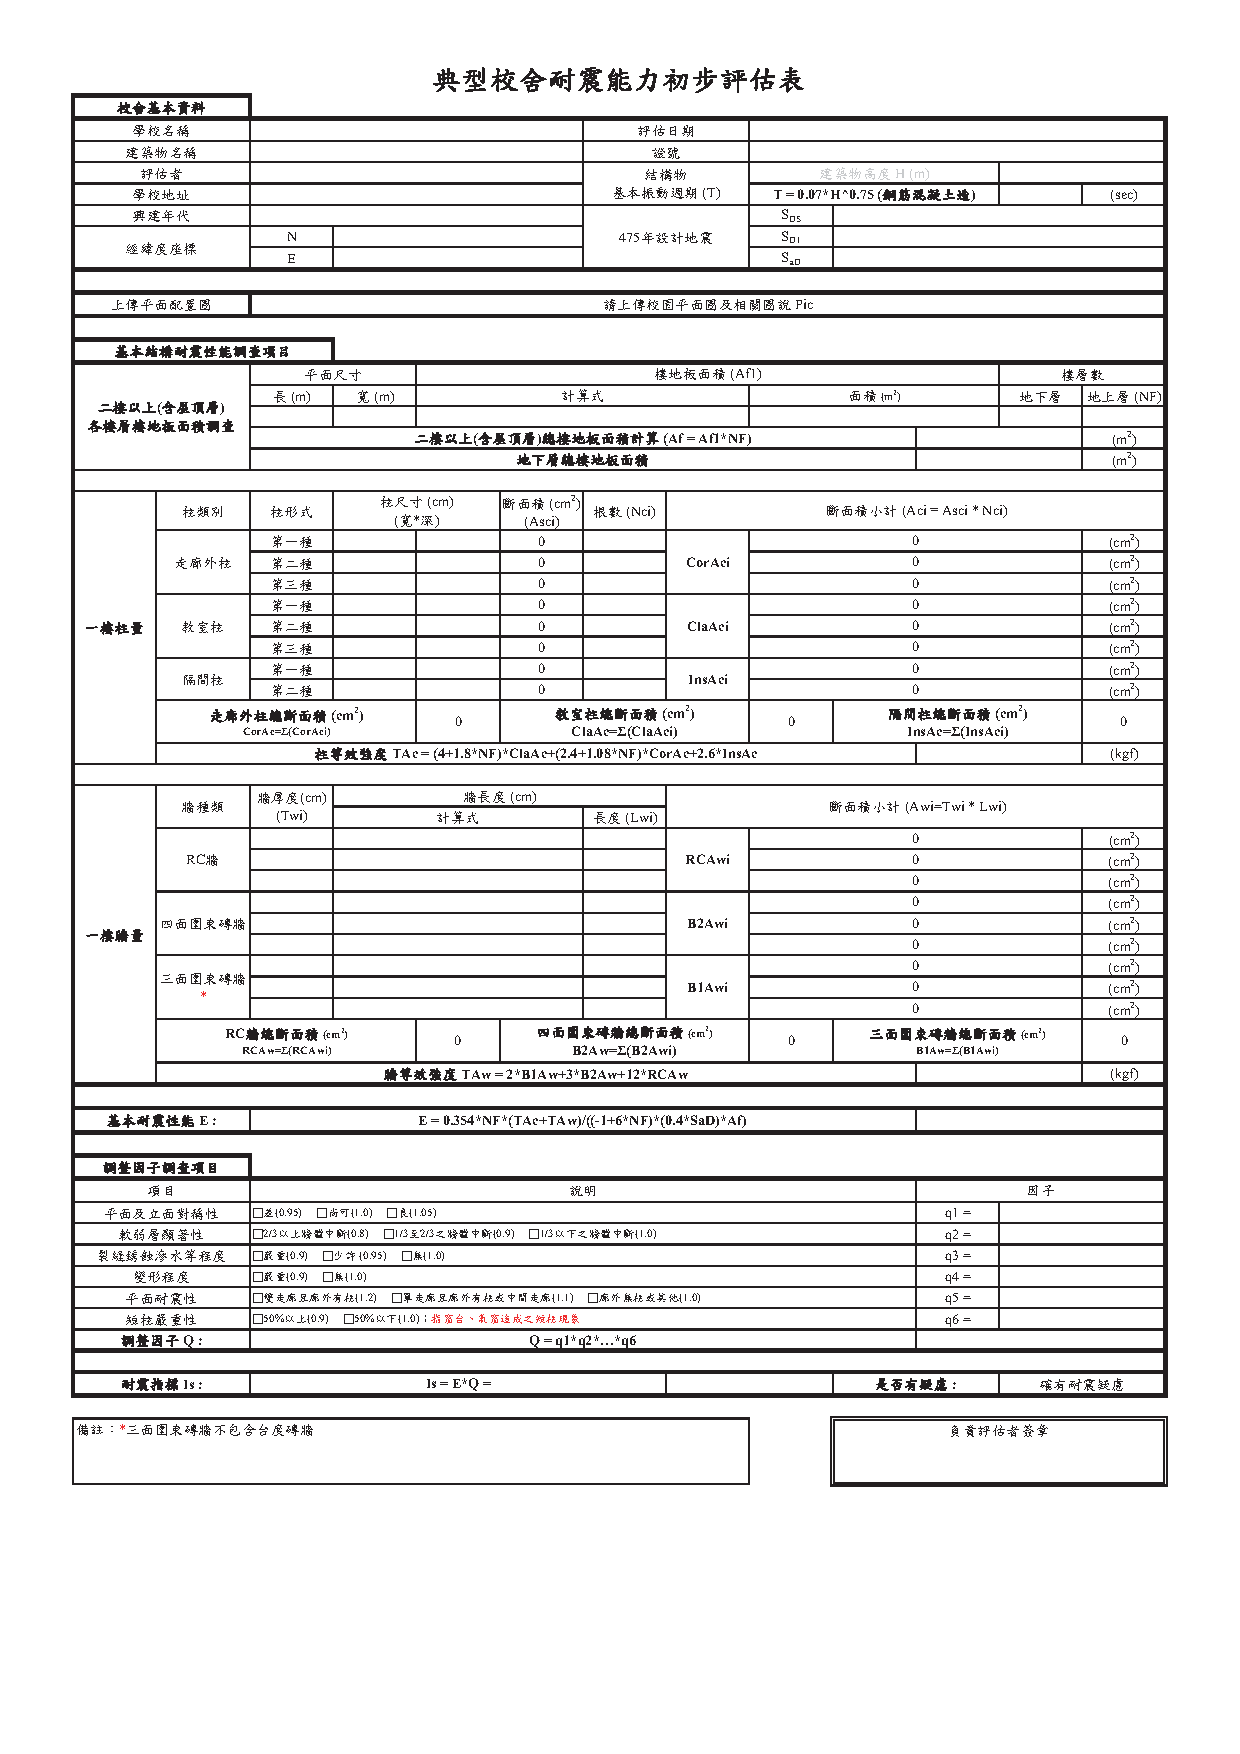
\includepdf[fitpaper=true,scale=0.95]{appendix/20120516-Preliminary-Typical.pdf}

%%% 如果有附錄二、三、...,則在此繼續加上「附錄編排」碼
% 每一個附錄會自動以新頁開始

\newpage
\chapter*{附錄二:典型校舍詳細評估表} % 修改附錄編號與你的附錄名
\label{appendix-de}
\addcontentsline{toc}{chapter}{附錄二:典型校舍詳細評估表} %建議此內容應與上行相同
\renewcommand{\thechapter}{二} % 如果是附錄二,則內容應為{二}

\setcounter{equation}{0} 
\setcounter{figure}{0} 
\setcounter{footnote}{0} 
\setcounter{section}{0} 
\setcounter{subsection}{0}
\setcounter{subsubsection}{0}
\setcounter{table}{0} 
%%% <<< 附錄編排碼 end

% 附錄內容開始
見下頁。

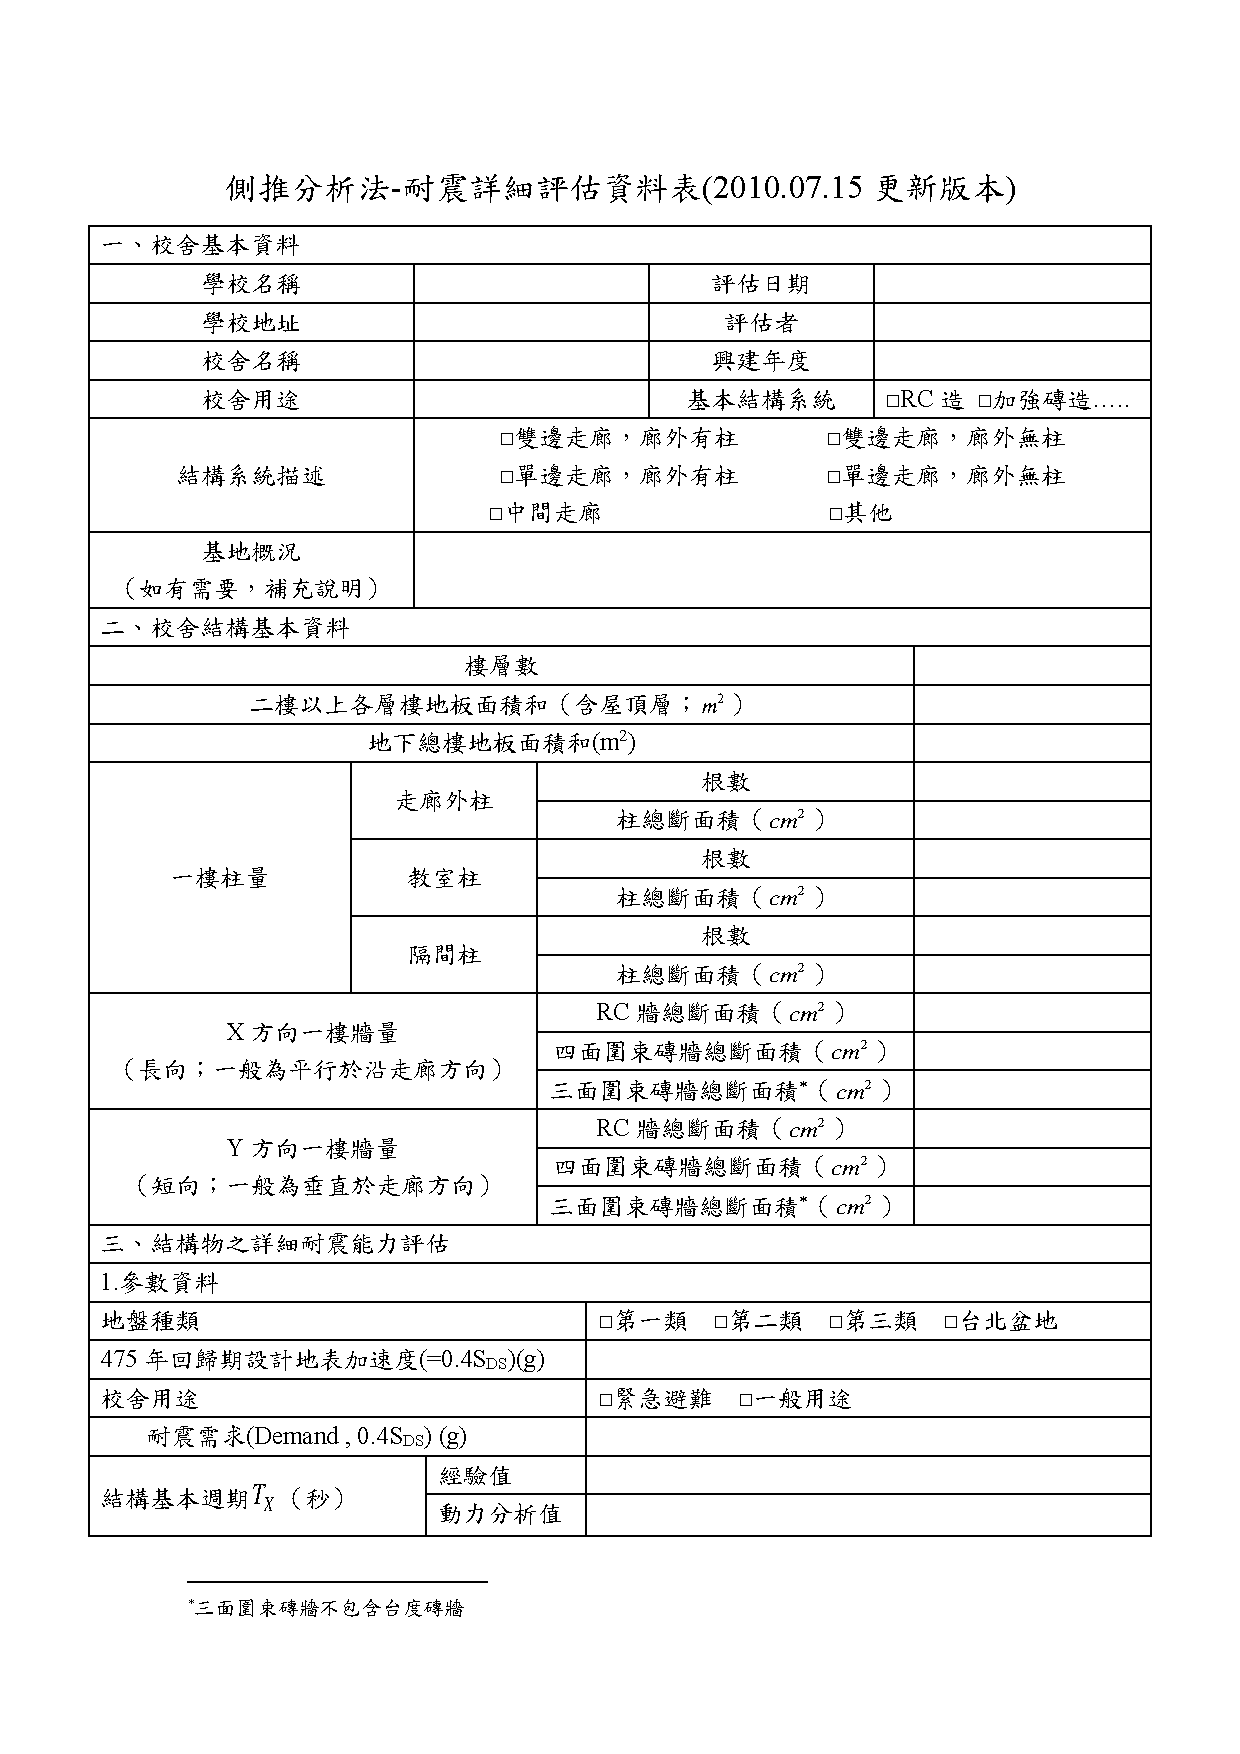
\includepdf[fitpaper=true,scale=0.95]{appendix/detailed-evaluation.pdf}


\newpage
\chapter*{附錄三:典型校舍補強設計表} % 修改附錄編號與你的附錄名
\label{appendix-re}
\addcontentsline{toc}{chapter}{附錄三:典型校舍補強設計表} %建議此內容應與上行相同
\renewcommand{\thechapter}{三} % 如果是附錄二,則內容應為{二}

\setcounter{equation}{0} 
\setcounter{figure}{0} 
\setcounter{footnote}{0} 
\setcounter{section}{0} 
\setcounter{subsection}{0}
\setcounter{subsubsection}{0}
\setcounter{table}{0} 
%%% <<< 附錄編排碼 end

% 附錄內容開始
見下頁。

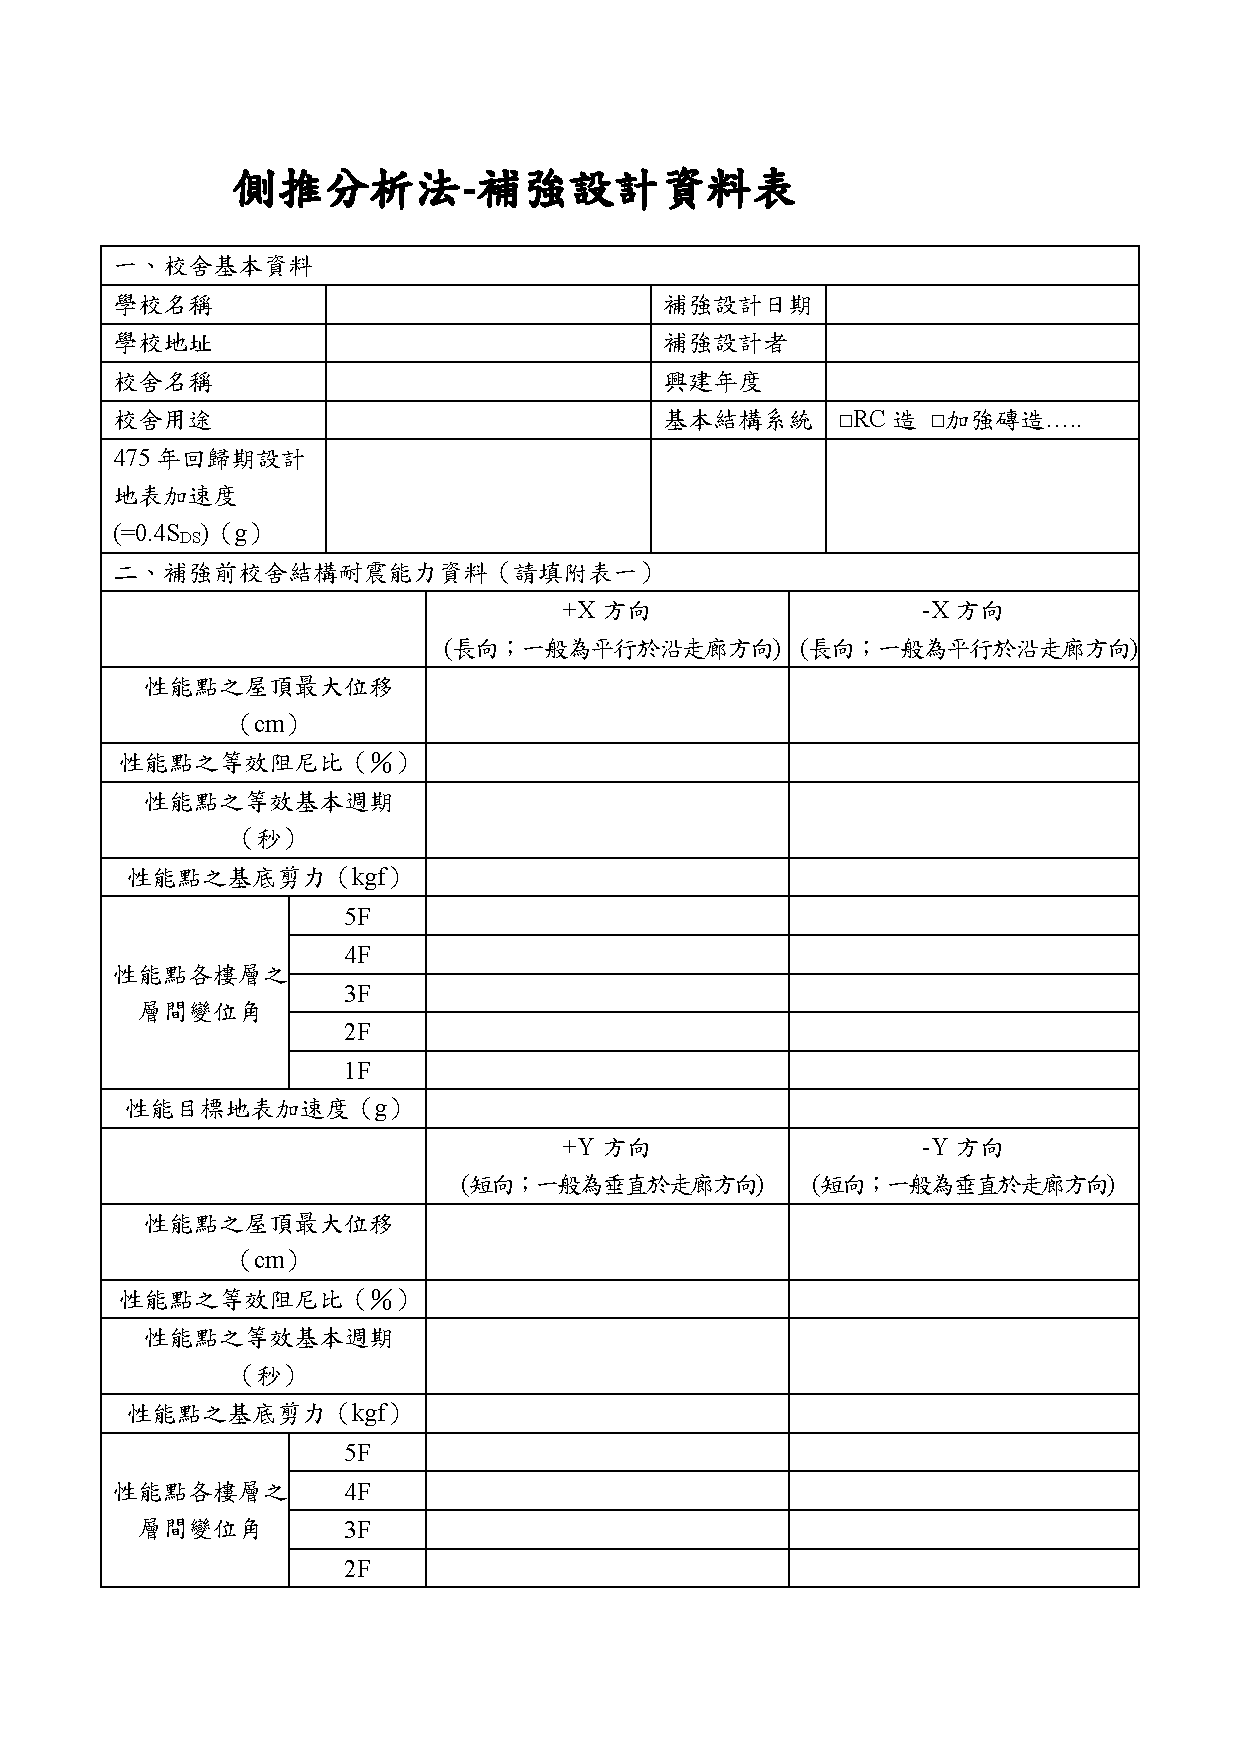
\includepdf[fitpaper=true,scale=0.95]{appendix/retrofit.pdf}



\newpage
\chapter*{附錄四:竣工資料上傳表} % 修改附錄編號與你的附錄名
\label{appendix-re}
\addcontentsline{toc}{chapter}{附錄四:竣工資料上傳表} %建議此內容應與上行相同
\renewcommand{\thechapter}{四} % 如果是附錄二,則內容應為{二}

\setcounter{equation}{0} 
\setcounter{figure}{0} 
\setcounter{footnote}{0} 
\setcounter{section}{0} 
\setcounter{subsection}{0}
\setcounter{subsubsection}{0}
\setcounter{table}{0} 
%%% <<< 附錄編排碼 end

% 附錄內容開始
見下頁。

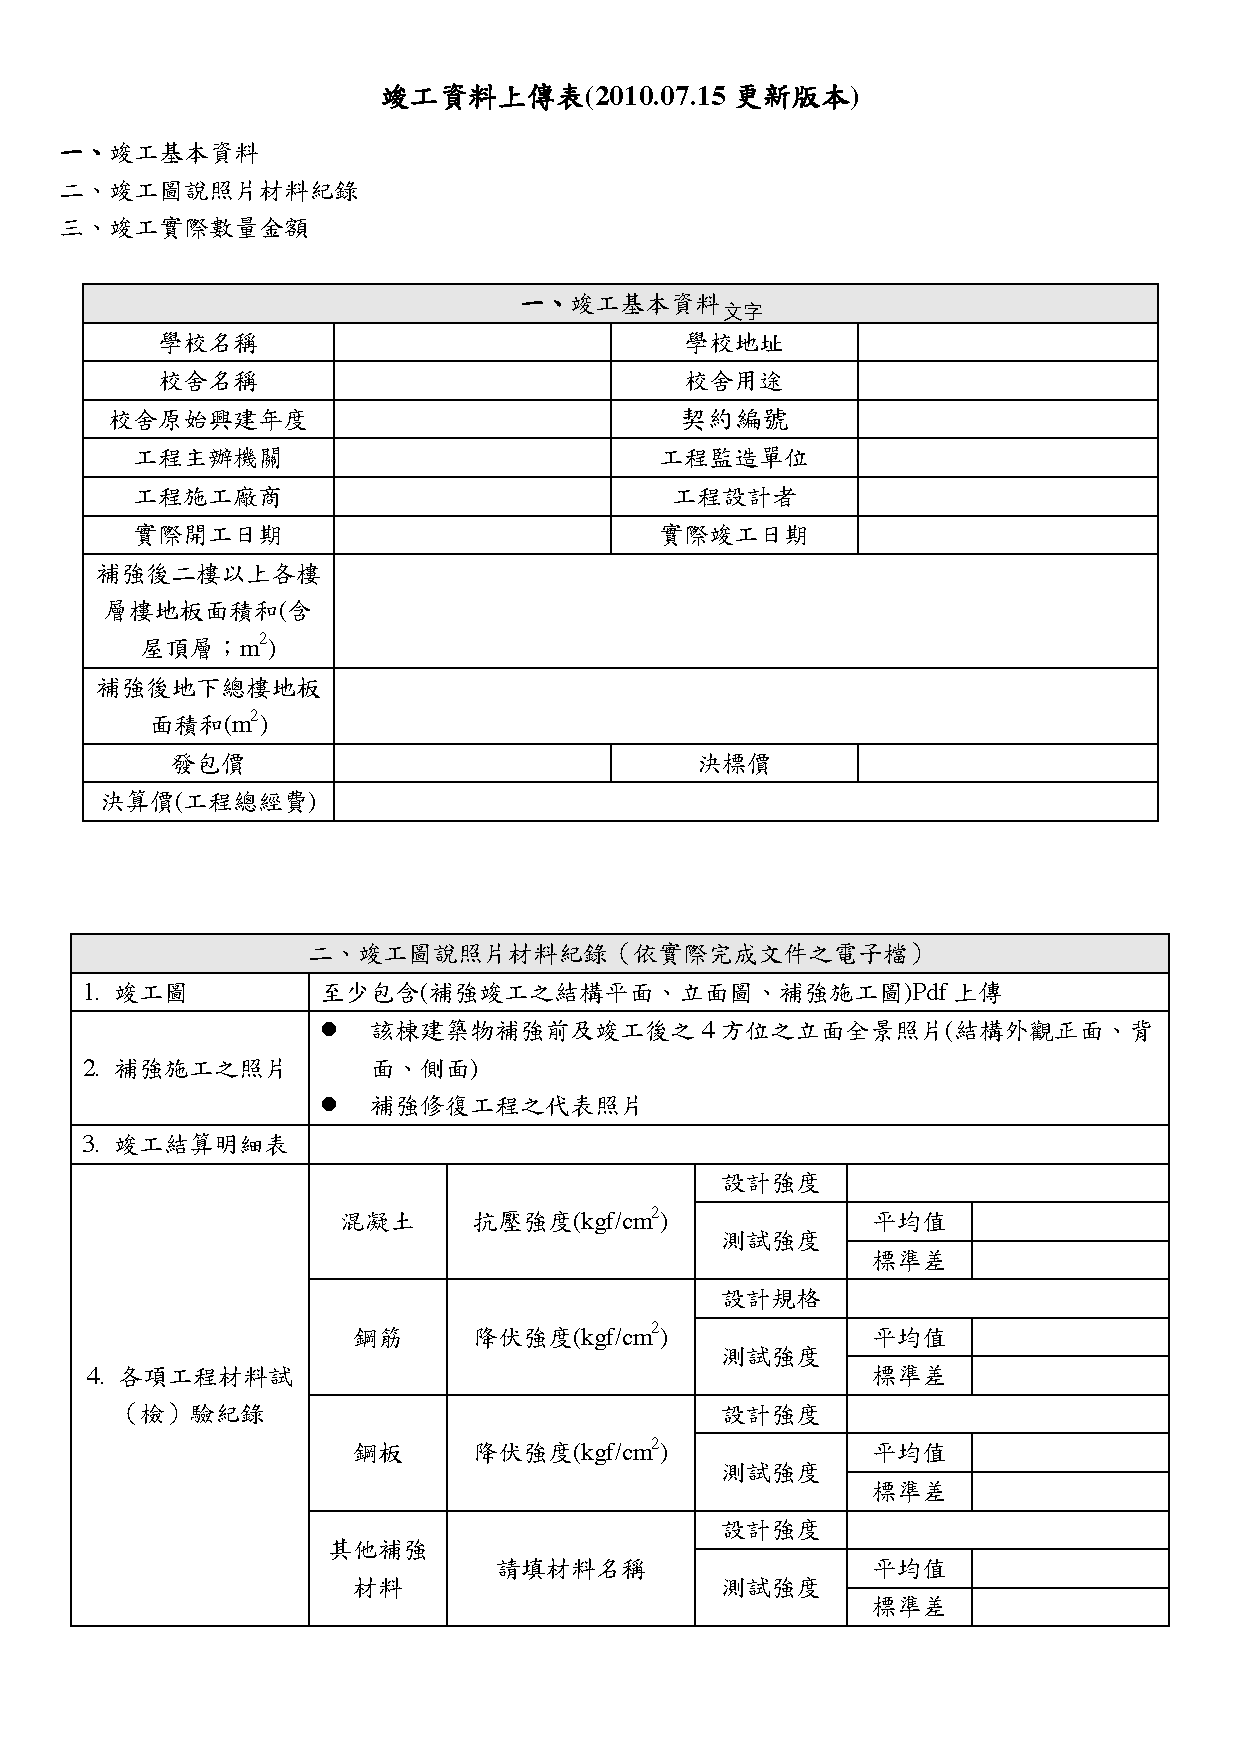
\includepdf[fitpaper=true,scale=0.95]{appendix/cob.pdf}


